
\section{Evaluation}
\label{sec:results}


\subsection{Experimental Setup}
\label{sub:experimentalSetup}

We have looked to several bug repositories like Bugzilla, Apache issue tracker,
Eclipse project issue tracker etc and noticed number of bugs with major, minor,
critical and blocker priorities. We took choose several bugs from them
considering couple of facts
\begin{mylist}

\item \textbf{Popularity}: How much it is used among the developers and
industries,
\item \textbf{Severity} : We consider major, critical and blocker priority bugs
only considering the facts at the bug affects dependent applications and other
libraries severely.
\item \textbf{Age and state} : We consider latest bugs which were reported in
the last 5 years.
We also consider such bugs which still remains un-fixed.

We did all the experiments in a laptop pc equipped with a dual core Intel i5
2.3-2.9 GHz processor, 8 GB or RAM, Microsoft Windows 8.1 operating system, JDK
version 1.7-45 with 2 GB of allocated heap space. All the bug reproduction was
done on
Eclipse Juno IDE. For static analysis and instrumentation we have used \soot\
version 2.5.0 and \soot\ \infoflow\ for static taint analysis. We have also used
java decompiler JD version 0.7.0.1. 

\end{mylist}

\subsection{Evaluation Matrices}
\label{sub:evaluationMartices}

We have conducted the evaluation based on the matrices which empirically
measures the precision and the performance of the developed tool. We measures
the precession in terms of the quality of the patch and some other criteria
listed bellow and the performance based on the time taken and the memory
footprint.

\begin{mylist}

\item \textbf{Patch similarity with the developers' patch} : This matrix is for
the qualitative analysis of our auto generated patches. By this measurement we
have not only ensure the effectiveness of the patch but also look at the
similarity of logic an patch construction with the developers' one.After the
patching we compared both the auto-generated patch code with the developer's
patching code we found in the bug repositories. In the case the bug is still
un-fixed we looked for the comments and discussion in the panel and collects
the information about the potential patch. At the first step, we visually
compared the patches to see how much they are similar and dissimilar with the
developers' patch. We than use the instrumented class files and place it to the
library archive replacing the buggy class files. We reproduced the similar test
cases of the bugs and used the automated patched version and later fixed version
of the same library to compare the results. In case the results are the
primitive
or string type we have printed the output in the console and compare them. In
case the output is some complex object we compare the properties of them. Apart
from the test cases to reproduce the bug, we also ran couple of good test case
to make sure that the patch is not behaving any other way. Based on this
experiment we made a metric named \textbf{Patch Quality Index (PQI)} which
can contains three values, high, medium and low where we consider high PSI being
a good close quality patch.

\item \textbf{Auto-generated patch size and the develops' patch size} : Apart
from the qualitative analysis we have measured quantitative aspect of the
Auto-generated patches and compared their sizes with the developers' one.
Quantitative measurement comes to picture only when we are satisfied with the
qualitative measurement. We came up with a metric called \textbf{Patch Size
Index (PSI)}. In case our patch is qualitatively satisfactory and the size is
less than the developer one the we assign PSI as high. In case the size varies
in $\pm5\%$ we assign PSI as medium. If our patch is more than $5\%$ bigger than
the develops' one then PSI is assigned to low.

\item \textbf{Already handled exception} : We have analyzed the call graph to
see higher in the call chain or in the same method if a particular statement is
handled or not. In such cases we have abort our patching effort considering that
the exception is caught with exact exception type or its base type. We have also
done measurement to see if the patching actually disrupts the normal program
flow or not and we made a metric called \textbf{Program Flow Consistency Index
(PFCI)} which is calculated as
$$PFCI = \frac{Patch_{HE}}{Stmt_{HE}}$$

where $Patch_{HE}$ = Total number of patch placed in already handled exceptions,
and $Stmt_{HE}$ =  total number of statements in the program which are already
handled and $0 \le PFCI \le 1$. The lower value of $PFCI$ is desirable.


\item \textbf{Cascaded exception} : Cascaded exception can be a result of 
auto-generated patching in the case the patched objects are used as a input
to other methods and violates the specification there. This is the limitation
in our technique in the some complicated cases where it requires develops' 
attention. The limitation is due to the fact that the analysis for the
repairing 
technique is a intra-procedural analysis and the constraint evaluation method is
very simple. For the constraint evaluation part, the solver is pluggable, we can
easily replace it with a third party solver. Cascaded exception can be noticed 
when the string object we are patching is generation some specific URI or driver
string which would be used to load or configure something. In such scenario, the
patch may produce some malformed string. In case there is a cascaded exception 
in string object, our analysis will take care of it, other wise it would abort. 

\item \textbf{Time} : For each of the analysis phase, we record the time taken.

\item \textbf{Memory Consumption} : Similarly we monitored memory consumption
for all of the phases in the analysis.

\end{mylist}

\subsection{Experimental Results}
\label{subsec:experimentalResults}

\begin{table}[t]
\centering
\scriptsize
\begin{tabular}{l|l}

\multicolumn{1}{c|}{\textbf{Notation}} &
\multicolumn{1}{c}{\textbf{Meaning}} \\

\hline
API & Analyzed library\\
BugID & Unique ID in bug repository\\
Priority & Severity of bug \\
$PQI$ & Program Quality Index\\
$PSI$ & Program Size Index\\
$PFCI$ & Program Flow Consistency Index\\
$\mathcal{N}_{Unit}$ & Total \#\code{Units} analyzed\\
$\mathcal{IC}_{NO}$ & Instrumentation without optimization\\
$\mathcal{IC}_{WO}$ & Instrumentation with optimization\\
$\mathcal{N}_{CG}$ & Size of the call graph\\
$\mathcal{PF}_{CA}$ & Profiling data of constraint analysis(sec/MB)\\
$\mathcal{PF}_{TA}$ & Profiling data of taint analysis(sec/MB)\\
$\mathcal{PF}_{CG}$ & Profiling data of call graph(sec/MB)\\
$\mathcal{PF}_{IN}$ & Profiling data of instrumentation phase(sec/MB)\\
$\mathcal{RS}_{CE}$ & If cascaded exception exists\\

\end{tabular}

\caption{Notations used in Table~\ref{tab:results}}
\label{tab:Notation}
\end{table}

\begin{table*}[t]
\setlength{\tabcolsep}{3pt}
\centering
\scriptsize
\begin{tabular}{l|l|l|l|l|c|c|c|c|c|c|c|c|c|c}
\multicolumn{1}{c|}{\textbf{API}} &
\multicolumn{1}{c|}{\textbf{BugID}} &
\multicolumn{1}{c|}{\textbf{Priority}} &
\multicolumn{1}{c|}{\textbf{$PQI$}} &
\multicolumn{1}{c|}{\textbf{$PSI$}} &
\multicolumn{1}{c|}{\textbf{$PFCI$}} &
\multicolumn{1}{c|}{\textbf{$\mathcal{N}_{Unit}$}} &
\multicolumn{1}{c|}{\textbf{$\mathcal{IC}_{NO}$}} & %instrumentation with
%optimization
\multicolumn{1}{c|}{\textbf{$\mathcal{IC}_{WO}$}} & %instrumentation without
%optimization
\multicolumn{1}{c|}{\textbf{$\mathcal{N}_{CG}$}} &
\multicolumn{1}{c|}{\textbf{$\mathcal{PF}_{CA}$}} & %profile for constraint
\multicolumn{1}{c|}{\textbf{$\mathcal{PF}_{TA}$}} & %profile for taint analysis
\multicolumn{1}{c|}{\textbf{$\mathcal{PF}_{CG}$}} & %profile for call graph
\multicolumn{1}{c|}{\textbf{$\mathcal{PF}_{IN}$}} & %profile for instrumentation
\multicolumn{1}{c}{\textbf{$\mathcal{RS}_{CE}$}}\\ % cascaded exception

\hline

\code{Aries} 	 	  			& \cite{ARIES1204}
 & Major   & High & Mid & $0$ &$129$ &$42$& $5$ & $3.5K$ & $3.1/10$ & $0.6/31$ &
$12.8/146$ &$2.3/142$ & $\checkmark$ \\

\code{Commons CLI2.x}  			& \cite{CLI46} 	   		  &
Major 	& Mid & Low & $0$ & $21$ & $13$ & $2$ & $3.2K$ & $2.8/5$ & $0.6/32$ & $12/212$ & $2/131$ & $\times$ \\

\code{Commons CLI1.x}  			& \cite{CLI193}    		  &
Major 	& High & Mid & $0$ & $53$ & $19$ & $19$ & $3.2K$ & $2.8/5$ & $0.5/30$ &
$11.6/149$ & $1.9/133$ & $\checkmark$ \\

\code{Commons Compress}			& \cite{COMPRESS26}		  &
Blocker & High & Mid & $0$ & $134$ & $46$& $4$ & $4K$ & $2.7/5$ & $0.5/30$ &
$11.5/209$ & $1.8/130$ & $\checkmark$ \\

\code{Commons IO}   			& \cite{IO179}  		  &
Major 	& High & Mid & $0$ & $125$ & $76$ & $1$ & $3.3K$ & $3/11$ & $0.5/33$ &
$12/209$ & $2/141$ & $\checkmark$\\

\code{Commons Lang} 	  		& \cite{LANG457}		  &
Major 	& High & Mid & $0$ & $240$ & $168$ & $8$ & $5.1K$ & $3/19$ & $0.57/30$ &
$16.5/209$ & $2.8/158$ & $\checkmark$ \\

\code{Commons Math} 	  		& \cite{MATH198} 		  &
Major 	& High & Mid & $0$ & $300$ & $36$ & $2$ & $3.4K$ & $3/20$ & $0.5/30$ &
$11.9/209$ & $2.9/152$ & $\checkmark$ \\

\code{Commons Net} 	  			& \cite{NET442}
 & Major   & High & Mid & $0$ & $14$ & $6$ & $1$ & $3.3K$ & $2.8/6$ & $0.5/33$ &
$11.4/212$ & $1.9/132$ & $\checkmark$ \\

\code{Commons VFS} 	  			& \cite{VFS338}
 & Major 	& High & Mid & $0$ & $$ & $$ & $$ & $$ & $$ & $$ & $$ & $$ &
$\checkmark$ \\

\code{Eclipse AspectJ} 			& \cite{EclipseBug333066} & Major
& High & Mid & $0$ & $39$ & $6$ & $1$ & $25K$ & $3.8/24$ & $0.5/34$ & $43.6/214$ & $1.6/156$ & $\checkmark$ \\

\code{Eclipse Aspectj Weaver} 	& \cite{EclipseBug432874} & Major 	& High &
Mid & $0$ & $50$ & $4$ & $1$ & $20.6K$ & $3.1/18$ & $0.6/34$ & $41.2/212$ & $1.6/142$ & $\times$ \\

\code{FlexDK 3.4} 		  			&\cite{SDK14417}
 & Minor 	& High & Mid & $0$ & $600$ & $207$ & $25$ & $6.3K$ & $4.8/40$ & $0.4/31$ & $12.9/209$ & $2.6/189$ &
$\checkmark$ \\

\code{Hama 0.2.0} 			  		&\cite{HAMA212}
  & Critical! 	& High & Mid & $0$ & $35$ & $28$ & $5$ & $3.7K$ & $2.6/5$ & $0.5/33$ & $14.4/210$ & $3.1/134$ &
$\checkmark$ \\

\code{Hive} 			  		&\cite{}
  & Major 	& High & Mid & $0$ & $$ & $$ & $$ & $$ & $$ & $$ & $$ & $$ &
$\checkmark$ \\

\code{HttpClient} 	  			&\cite{HTTPCLIENT150}	  &
Major 	& High & Mid & $0$ & $14$ & $6$ & $1$ & $3.3K$ & $2.8/6$ & $0.5/33$ & $12.3/212$ & $2.7/131$ &
$\checkmark$ \\

\code{jUDDI} 	  				&\cite{JUDDI292}
 & Major 	& High & Mid & $0$ & $70$ & $10$ & $2$ & $3.2K$ & $3.1/11$ & $0.5/34$ & $13.6/209$ & $2.9/138$ &
$\checkmark$ \\

\code{Log4j} 		  			&\cite{ApacheLog4jBug}	  &
Major 	& High & Mid & $0$ & $17$ & $6$ & $1$ & $3.2K$ & $2.8/4$ & $0.5/32$ & $13/212$ & $2.5/131$ &
$\checkmark$ \\

\code{Qpid} 			  		&\cite{}
  & Blocker & High & Mid & $0$ & $$ & $$ & $$ & $$ & $$ & $$ & $$ & $$ &
$\checkmark$ \\

\code{Servicemix-soap} 			&\cite{SMXCOMP156}		  &
Major   & High & Mid & $0$ & $$ & $$ & $$ & $$ & $$ & $$ & $$ & $$ &
$\checkmark$ \\

\code{SOAP} 			 		&\cite{SOAP130}		      &
Major 	& High & Mid & $0$ & $165$ & $32$ & $5$ & $5K$ & $3.4/19$ & $0.6/30$ & $14/209$ & $2.3/148$ &
$\checkmark$ \\

\code{Struts2} 		  			&\cite{WW650}
 & Major 	& High & Mid & $0$ & $80$ & $25$ & $2$ & $16K$ & $3/14$ & $$0.5/32 & $25.9/210$ & $1.3/140$ &
$\checkmark$ \\

\code{Tapestry 5} 		  		&\cite{TAP51770}
 & Major 	& High & Mid & $0$ & $71$ & $31$ & $5$ & $6.2K$ & $2.9/10$ & $0.5/34$ & $22.3/211$ & $1.9/136$ &
$\checkmark$ \\

\code{Wicket} 		  			&\cite{WICKET4387}
 & Major 	& High & Mid & $0$ & $68$ & $16$ & $1$ & $70K$ & $3/14$ & $0.5/32$ & $52.4/210$ & $1.4/142$ &
$\checkmark$ \\

\code{XalanJ2} 		  			&\cite{XALANJ836}
 & Major 	& High & Mid & $0$ & $33$ & $13$ & $2$ & $3.3K$ & $2.7/8$ & $0.5/33$ & $13.5/213$ & $2.2/131$ &
$\checkmark$ \\

\end{tabular}

\caption{Experimental results}
\label{tab:results}
\end{table*}

In the table~\ref{tab:results} we have listed the data we got \tool\. We have
conducted our expriment over number of
bugs related to \java\ \code{String} API. We have used these notations in the
table which are explained


\begin{figure}[t]
\centering
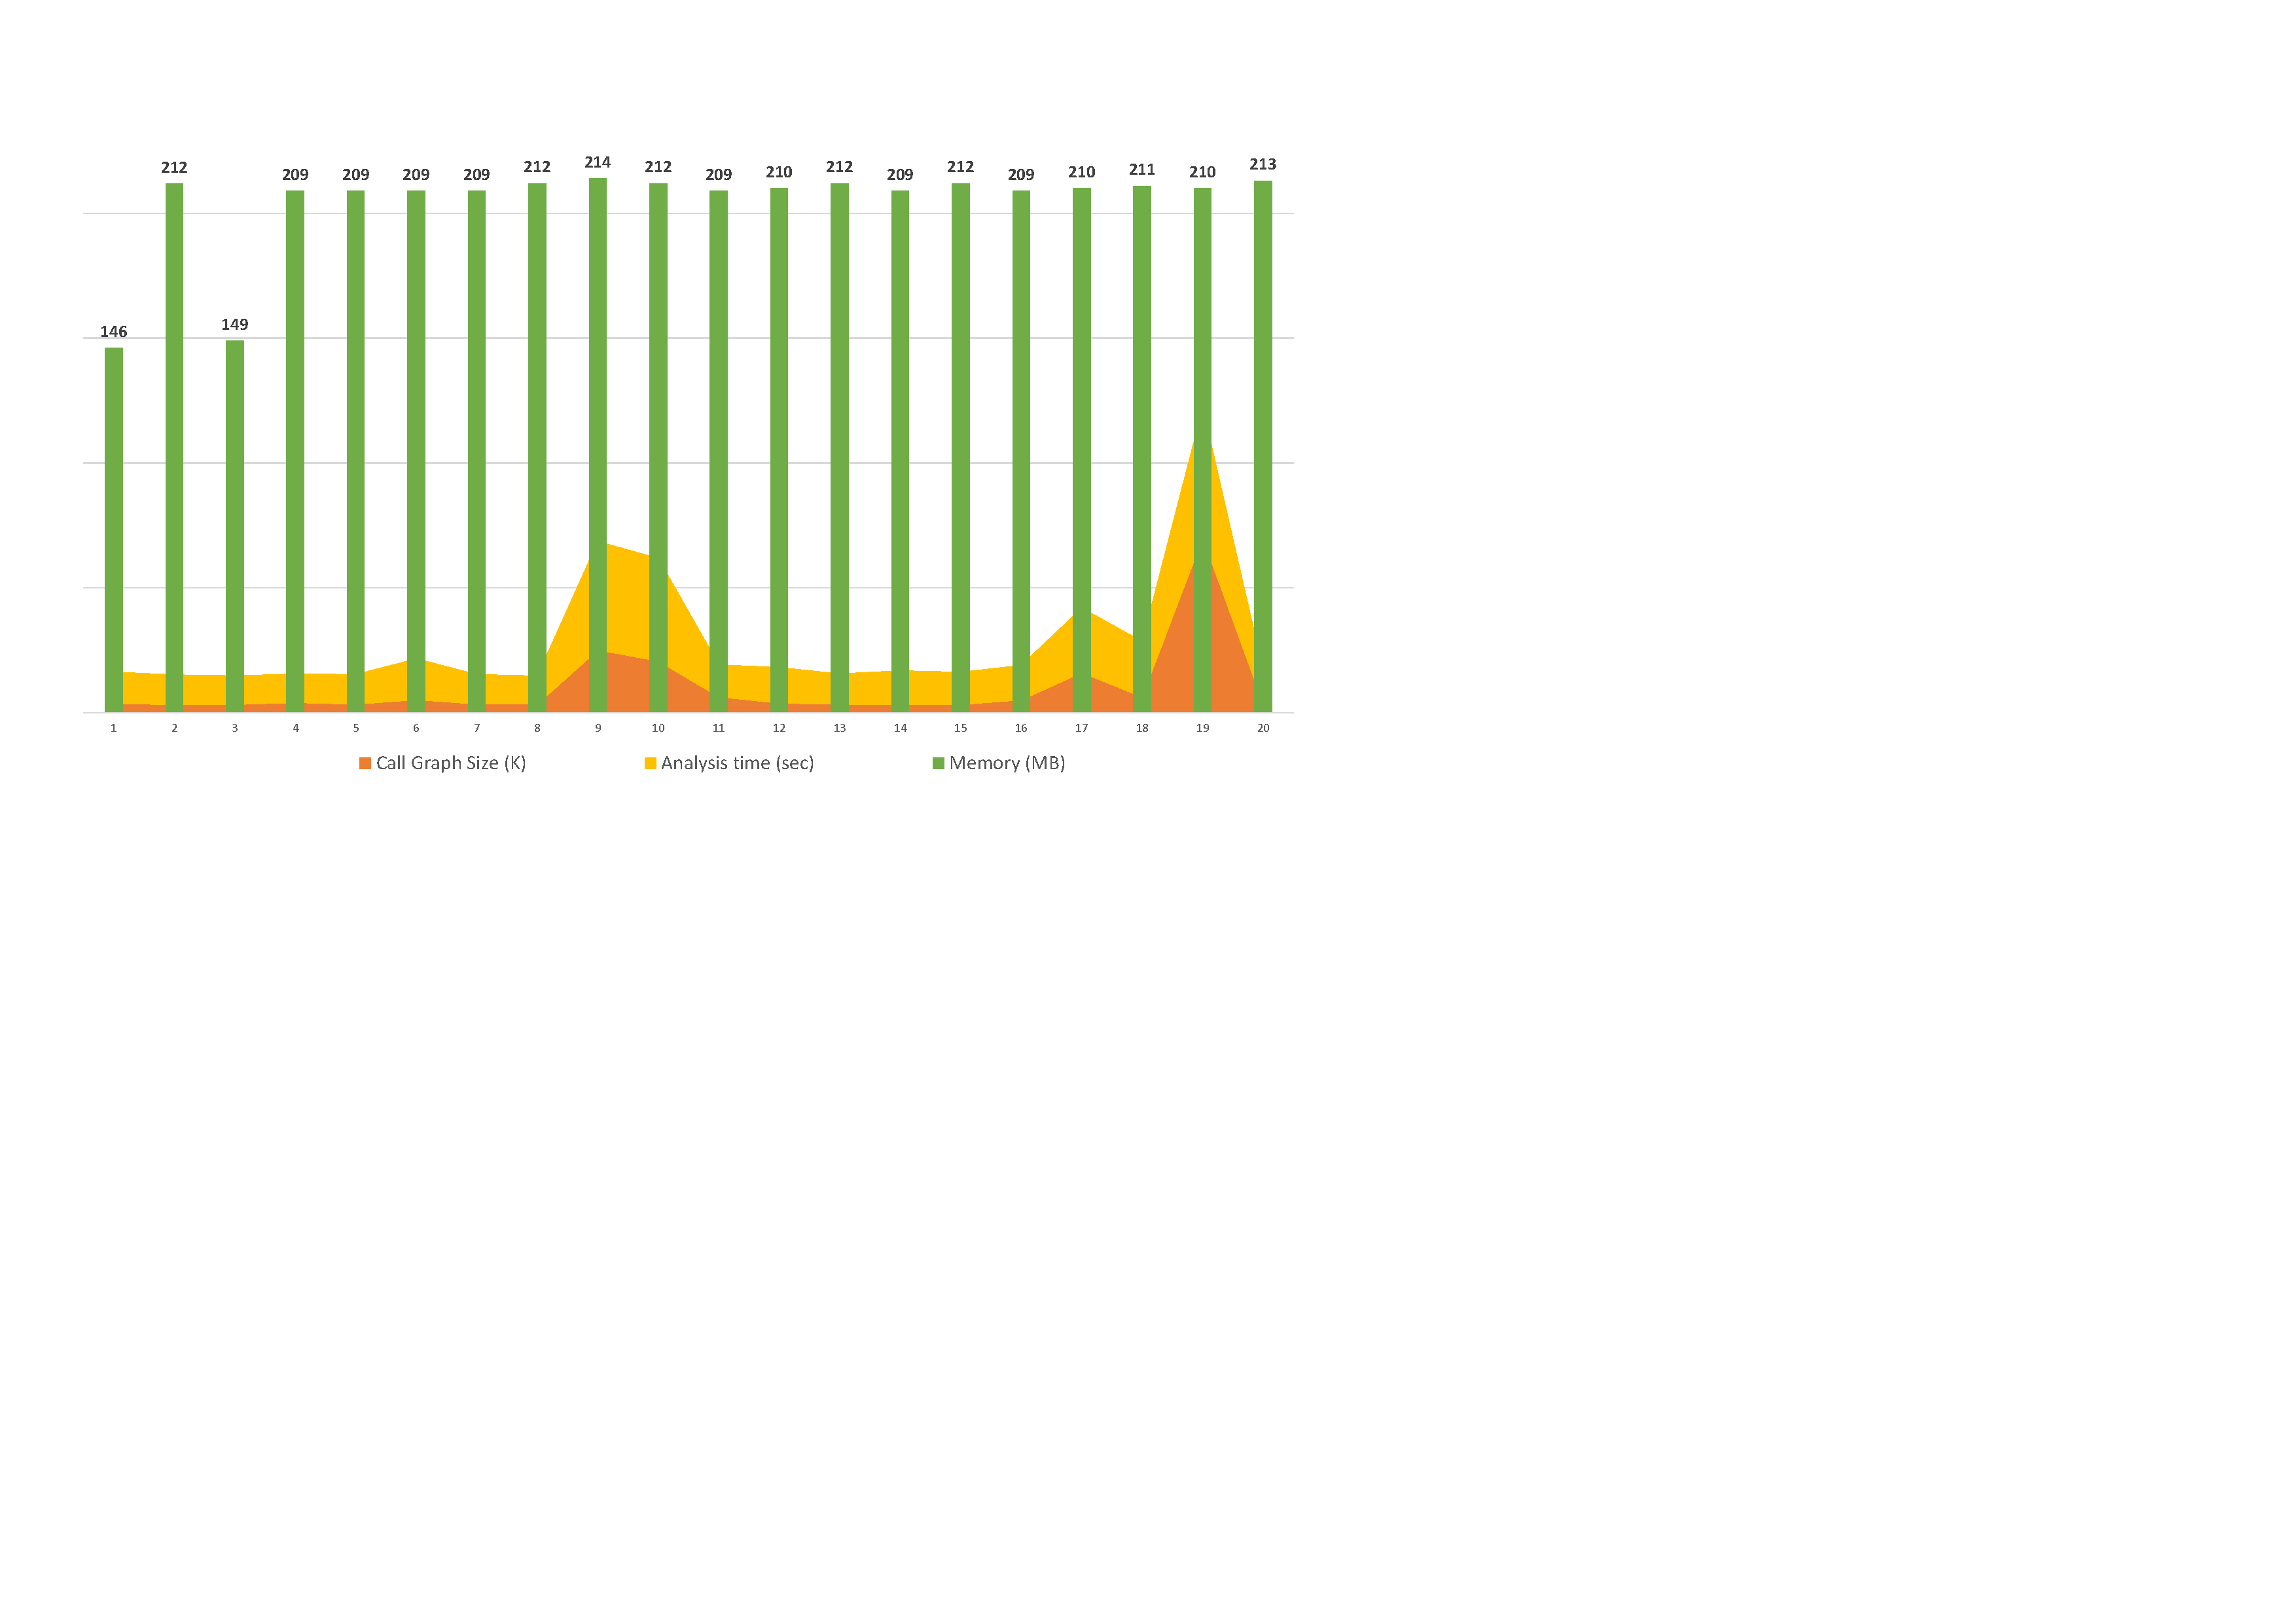
\includegraphics[scale = .3]{images/CallGraphHisto.pdf}
\caption{Performance statistics of call graph analysis phase}
\label{fig:callGraphHisto}
\end{figure}


\begin{figure}[t]
\centering
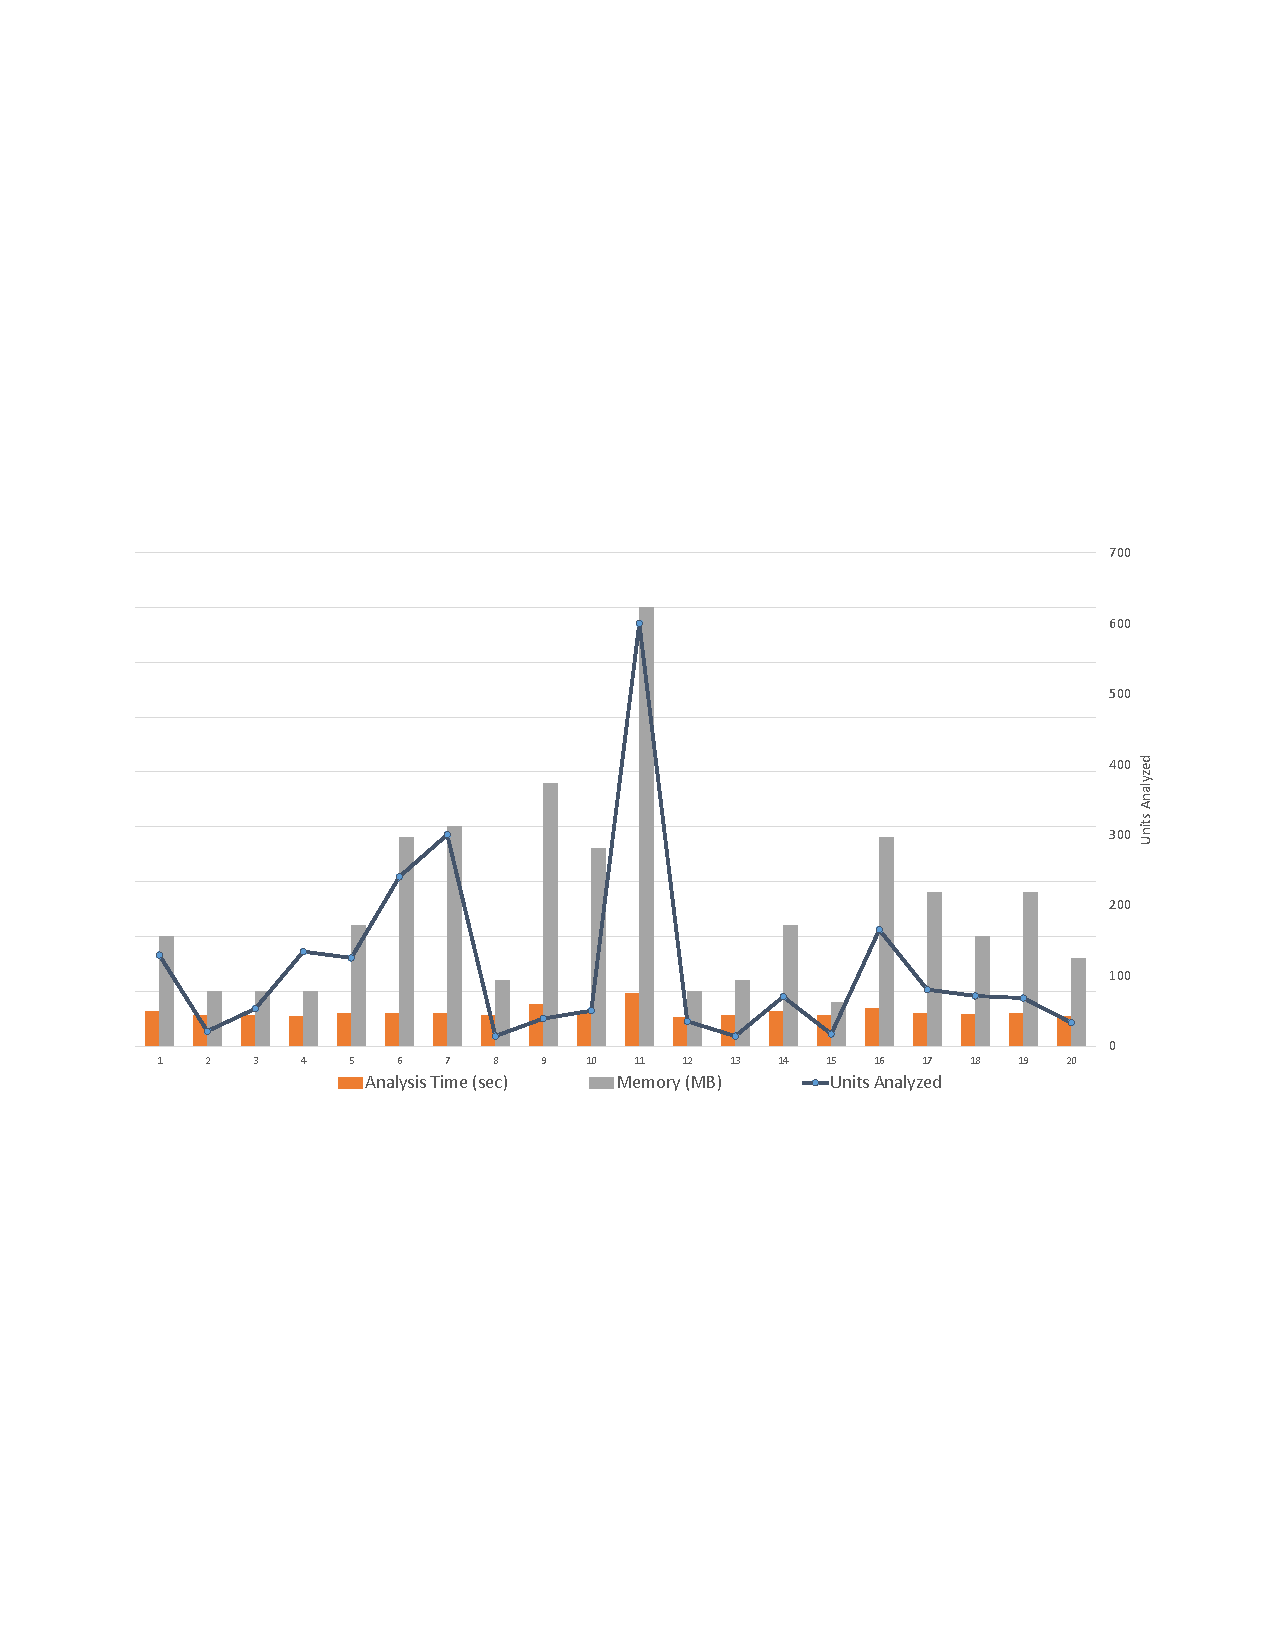
\includegraphics[scale = .5]{images/ConstraintHisto.pdf}
\caption{Performance statistics of constraint analysis phase}
\label{fig:constraintHisto}
\end{figure}



% \begin{figure}
%         \centering
%         \begin{subfigure}[b]{0.3\textwidth}
%                 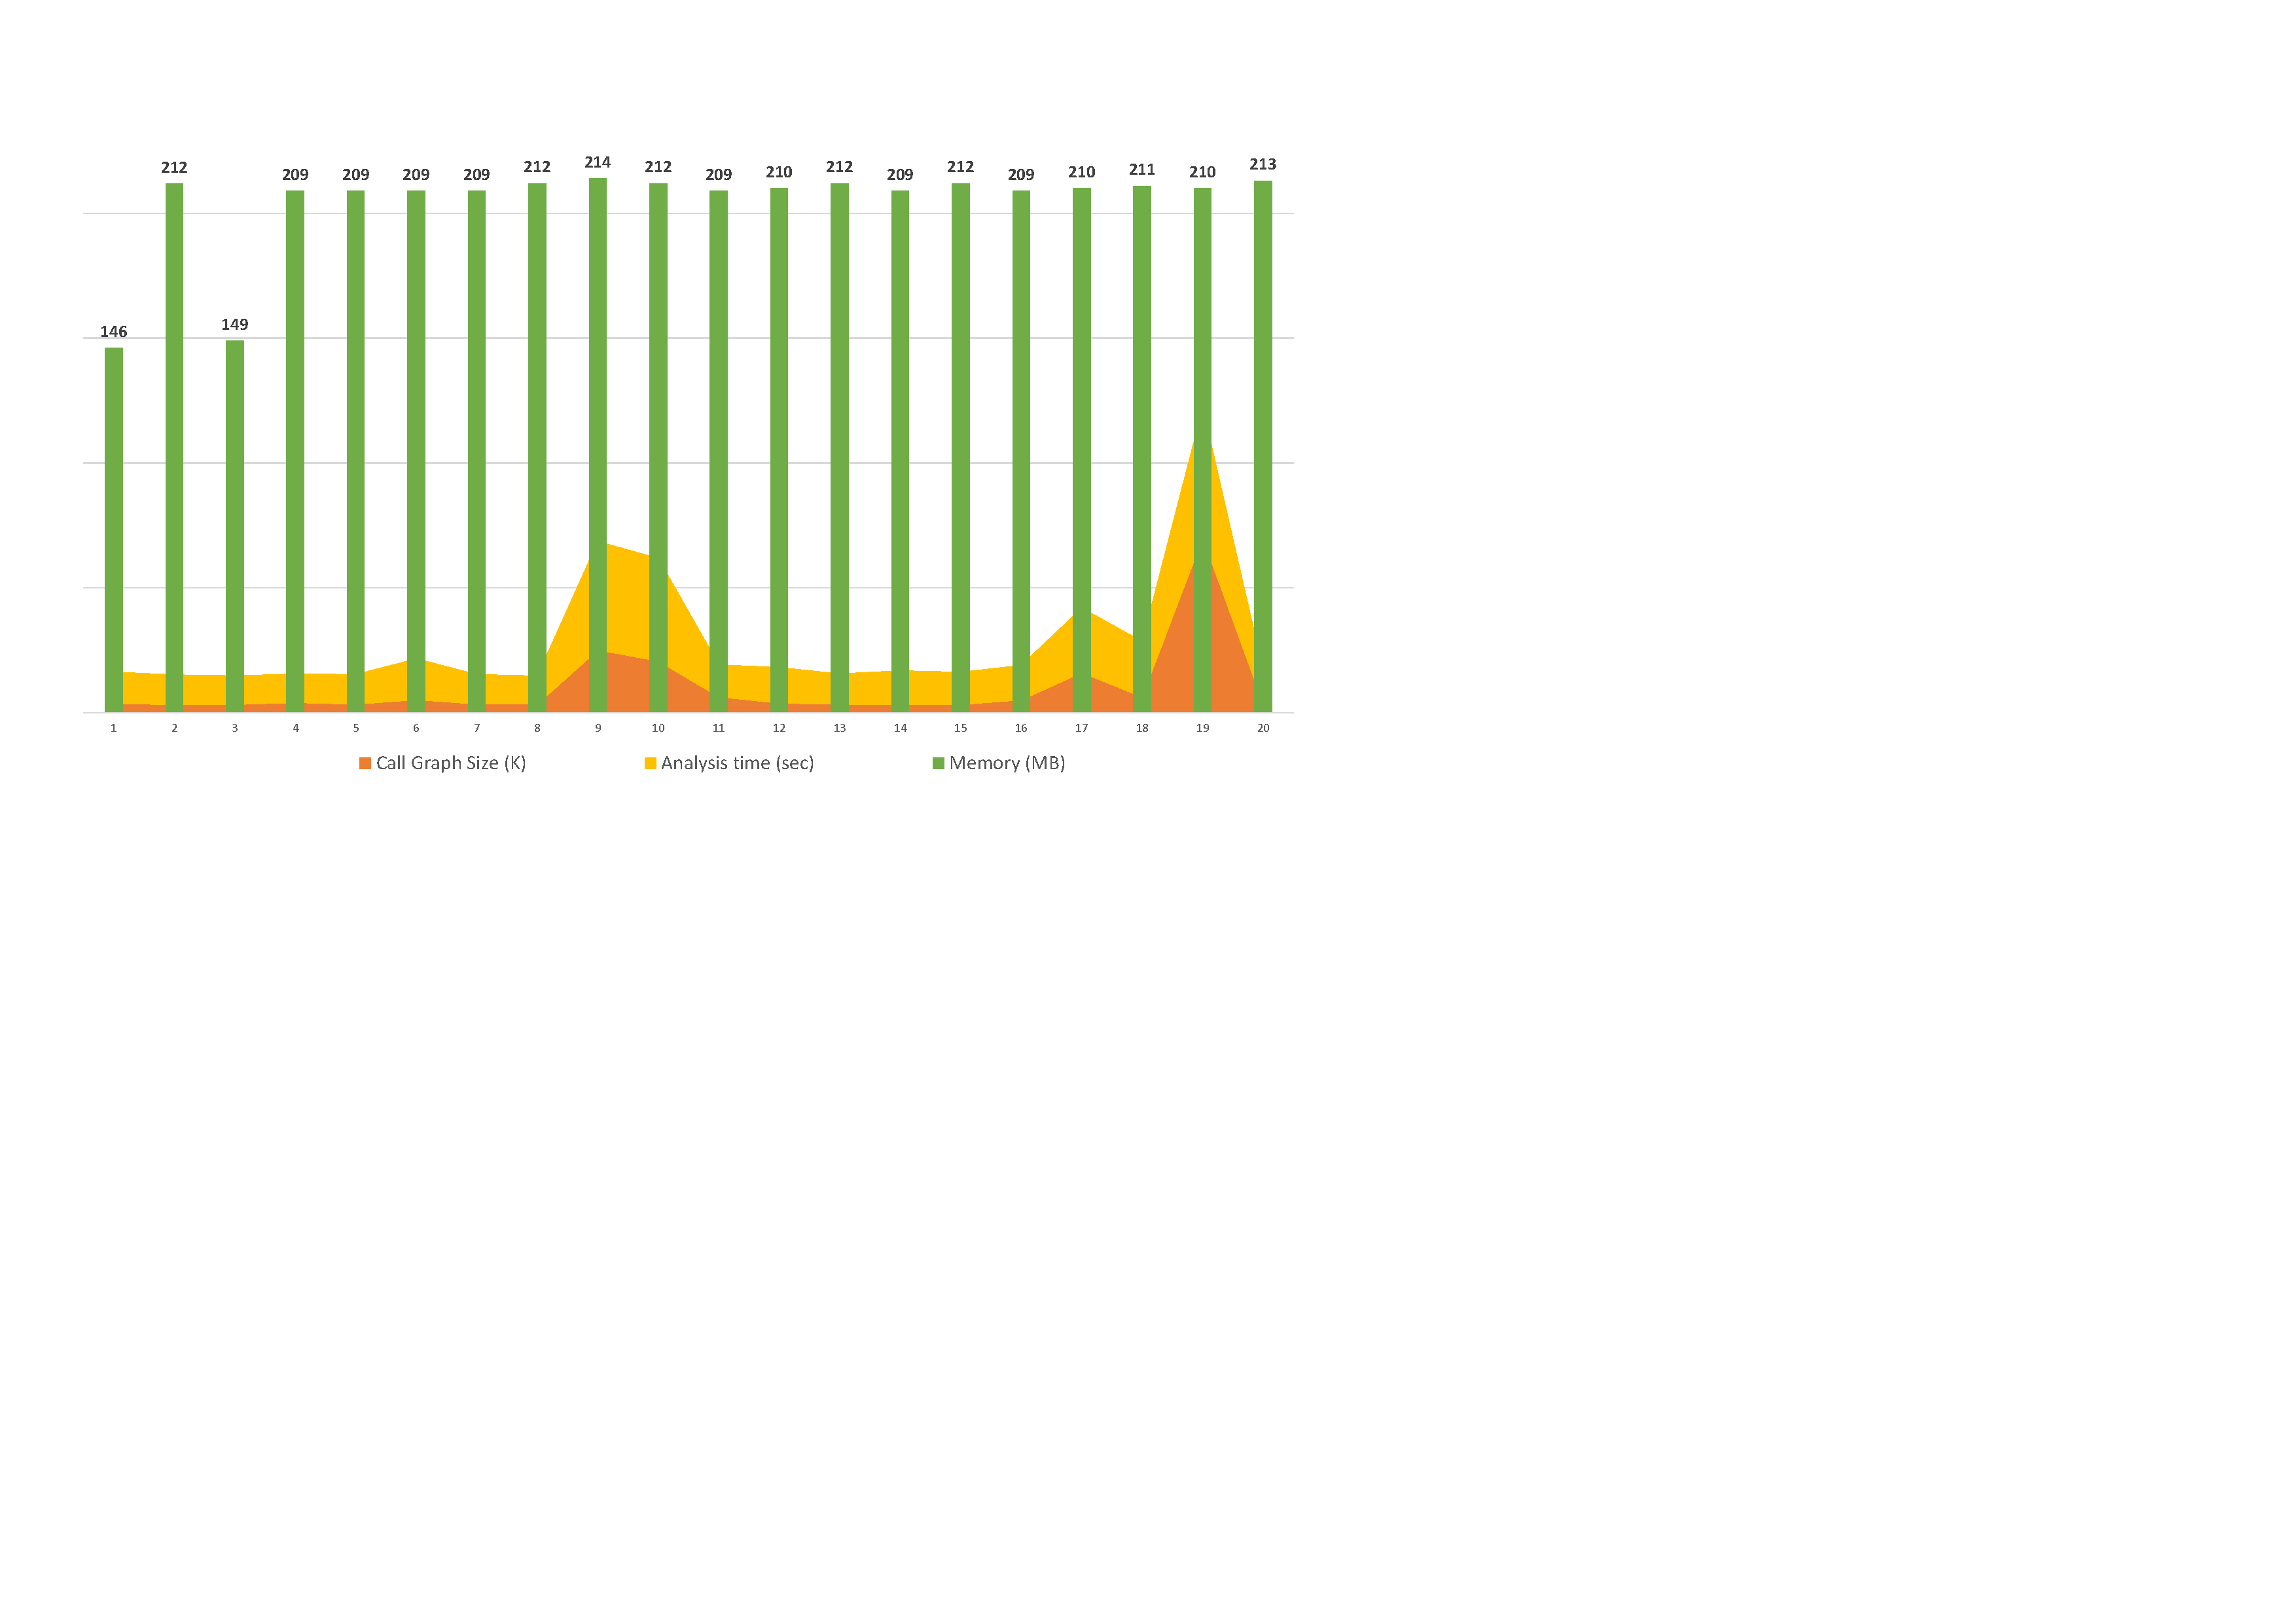
\includegraphics[width=\textwidth]{images/CallGraphHisto.pdf}
%                 \caption{A gull}
%                 \label{fig:gull}
%         \end{subfigure}%
%         ~ %add desired spacing between images, e. g. ~, \quad, \qquad, \hfill etc.
%           %(or a blank line to force the subfigure onto a new line)
%         \begin{subfigure}[b]{0.3\textwidth}
%                 \includegraphics[width=\textwidth]{tiger}
%                 \caption{A tiger}
%                 \label{fig:tiger}
%         \end{subfigure}
%         ~ %add desired spacing between images, e. g. ~, \quad, \qquad, \hfill etc.
%           %(or a blank line to force the subfigure onto a new line)
%         \begin{subfigure}[b]{0.3\textwidth}
%                 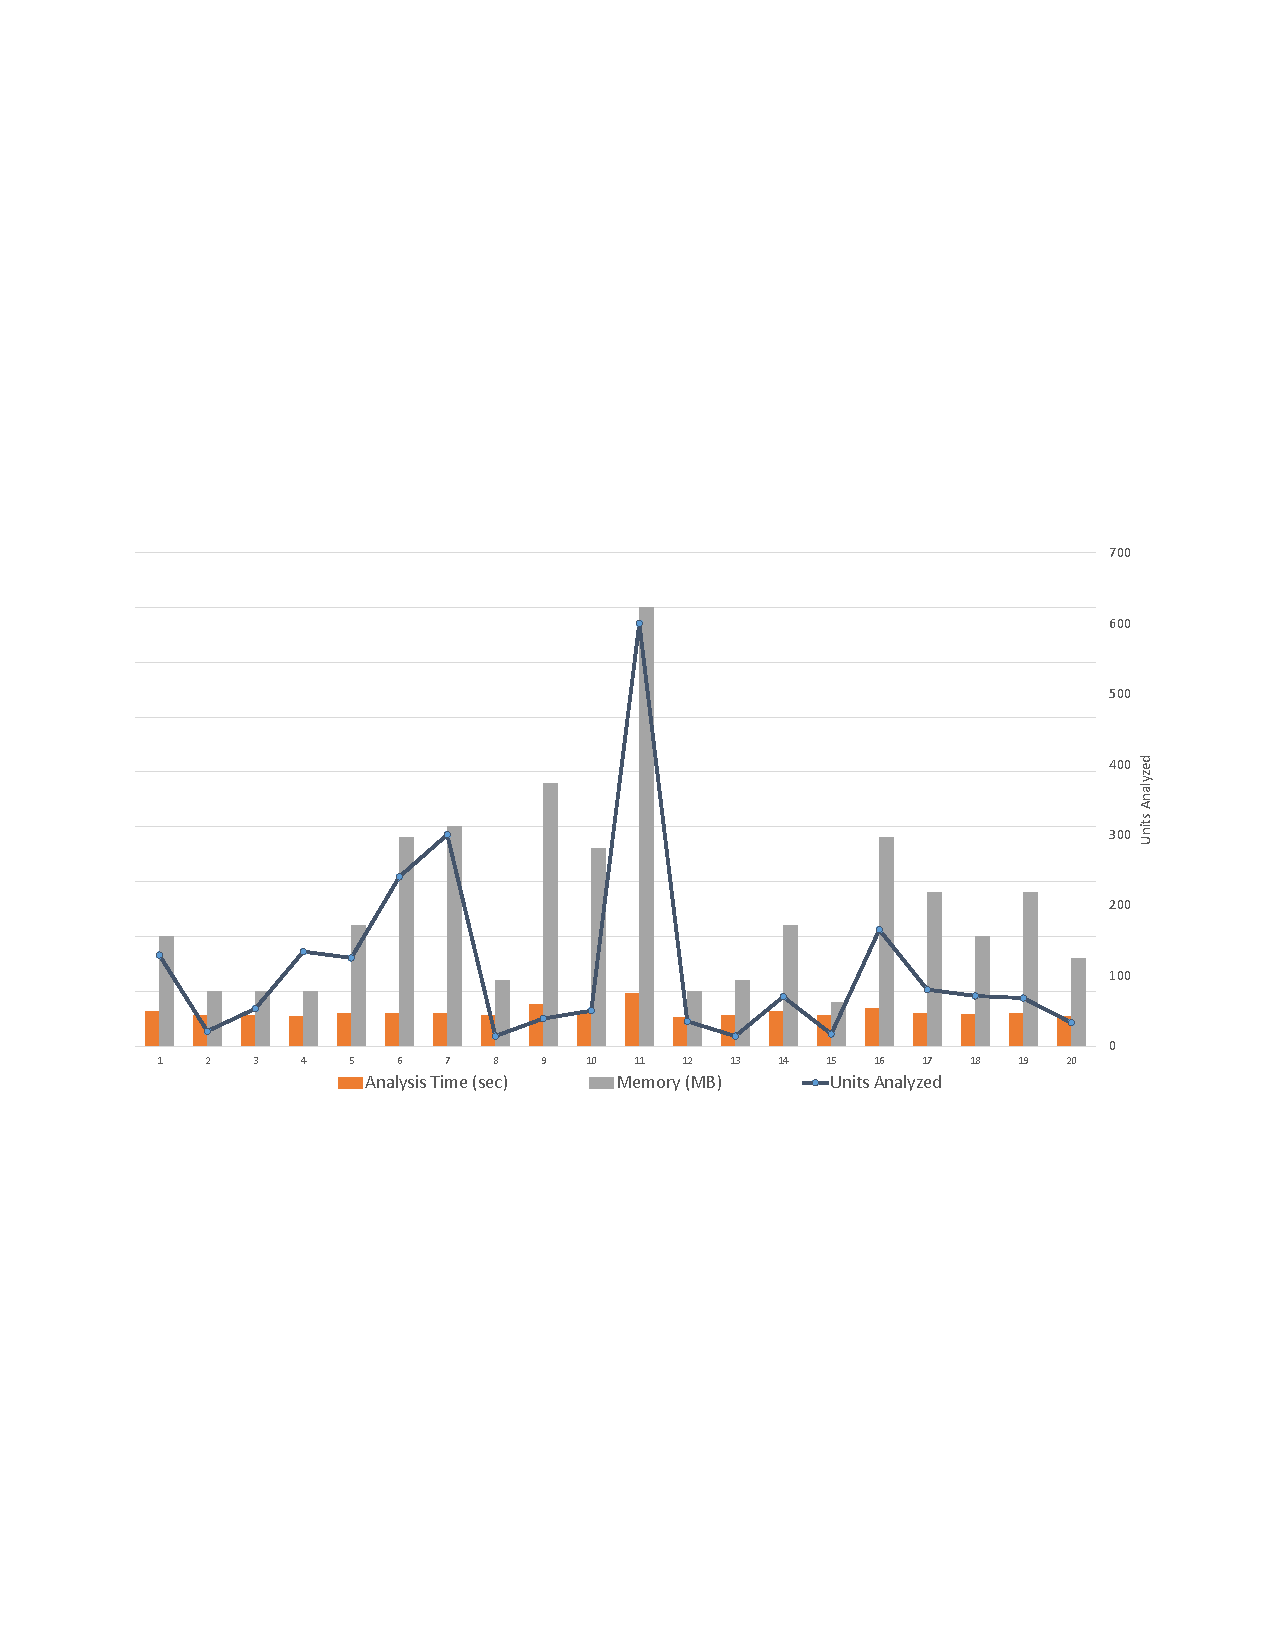
\includegraphics[width=\textwidth]{images/ConstraintHisto.pdf}
%                 \caption{A mouse}
%                 \label{fig:mouse}
%         \end{subfigure}
%         \caption{Pictures of animals}\label{fig:animals}
% \end{figure}